\documentclass[../main.tex]{subfiles}

\graphicspath{{\subfix{../images/}}}
\begin{document}
\chapter{First GraphQL application using Spring Boot}

\section{Setting up a Spring boot GraphQL Server}
Based on the concepts used in an application, other dependencies are also used. Some of them are:
\begin{itemize}
  \item {\textbf{\lstinline{spring-boot-starter-jpa}} is used to connect our application with data bases in an efficient manner. This dependency internally uses spring-data-jpa dependency.}
  \item {\textbf{\lstinline{mysql-connector-j}} provides a driver connectivity between our Java application and mysql data base. This dependency provides a Type-4 driver connectivity.}
  \item {\textbf{\lstinline{spring-boot-starter-websocket}} establishes a connection between a Client and Server to communicate. This connection requires in Subscription like applications.}
  \item {\textbf{\lstinline{spring-webflux}} publishes the data on User interface. To do this, GraphQL uses Mono, Publisher like classes.}
\end{itemize}
\printglossaries
\section{Writing GraphQL schema}
Once done with adding the GraphQL related libraries, we need to create GraphQL schema. Writing GraphQL schemas are quite easy, and they are portable across for promoting reusability. It becomes possible to write schemas with GraphQL’s own language which is nothing but \gls{SDL}.
The schema that we write for our application will contain the functionalities and the types that are being exposed by the application. In short, this schema can be considered as a contract between the client and the server that exposes the services.
GraphQL Tools library processes the GraphQL Schema files in order to build the correct structure. Once after building, wires special beans to this structure. There is no special configuration needed to register this schema as graphql-spring-boot-starter automatically detects this schema file.
\begin{lstlisting}[language=GraphQL, caption={Sample SDL}, label={lst:sample-sdl}]
  type Query 
  {
    message: String
  }
\end{lstlisting}
As our project holds a very simple service for exposure, the schema that we have written looks simple too. Otherwise, the schema will consist of the user-defined types that can be exposed. For example, Employee.
\begin{lstlisting}[language=GraphQL, caption={Employee SDL schema}, label={lst:employee-sdl-schema}]
  type Employee
  {
    id: ID! #non-nullable
    name: String
  }
  type Query
  {
    employees:[Employee]
  }
\end{lstlisting}
Also, the schema can hold type, mutations, and subscriptions.
The schema file that we write for a GraphQL application should be saved with graphqls extension (\lstinline{.graphqls}) and can be available anywhere on the classpath.
Let's create a folder named graphql under resources and place this schema file of extension, graphqls.

\begin{figure}[h!]
  \centerline{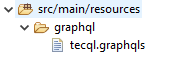
\includegraphics[width=150mm]{g11610443690953.PNG}}
  \caption{Spring boot structure to store graphql queries}
  \label{fig:Spring-boot-structure-to-store-graphql-queries}
\end{figure}

\subsection{Writing Resolvers}
We have added the GraphQL related dependencies to our spring boot project and defined a query that can fetch a String literal. Is there anything else to be done? 
Yes, we need to create a resolver.
The need for the resolver is to handle the various fields being mentioned in the type, query or mutation of the schema file (.graphqls file). 
Mutation is not covered yet and shall be covered later in this course.
Resolvers are the ones that can resolve the things that are present in the GraphQL schema.
So, the query that we have in the schema should have a resolver associated.
We shall create a query resolver by using annotation \lstinline{SchemaMapping}, which takes two parameters - \lstinline{typeName} and \lstinline{field}.
Out of these two parameters, \lstinline{typeName} is mandatory and field is optional.
The typeName parameter takes Query/Mutation/Subscription/any user-defined type. 
Have a look at the resolver that we have created for our GraphQL project.

\begin{lstlisting}[language=java, caption={Resolver example}, label={lst:resolver-example}]
  //package and import statements

  @Controller
  public class QueryResolver {

    @Autowired
    private Services service;

    @SchemaMapping(typeName="Query",field="message")
    public String getMessage() {
      return service.getMessage();
    }

  }

\end{lstlisting}
It is always very important to name the methods of the resolver using the field names available in the query.
In simple words, there should be a one-to-one correspondence between the fields of the query and the methods of the resolver.
The naming convention for the methods of the resolver can be either of the following.

\begin{itemize}
  \item field
  \item isField (if the return type is boolean)
  \item getField
\end{itemize}

Also, the method should return the type being available for the field in the query.
Now, take a look at the signature of the resolver method

\begin{lstlisting}[language=java]
  public String getMessage( )
\end{lstlisting}

that we have written for the type, query in the GraphQL schema. 

\begin{lstlisting}[language=GraphQL]
  type Query
  {
    message: String
  }
\end{lstlisting}

The resolver has got a method named \lstinline{getMessage()} for the field message in the Query and the return type of the method is String as the field message is of type String.
\begin{lstlisting}[language=XML]
  <dependency>
    <groupId>org.springframework.boot</groupId>
    <artifactId>spring-boot-starter-graphql</artifactId>
   </dependency>
  <dependency>
    <groupId>org.springframework.boot</groupId>
    <artifactId>spring-boot-starter-web</artifactId>
  </dependency>
  <dependency>
    <groupId>org.springframework.boot</groupId>
    <artifactId>spring-boot-starter-test</artifactId>
    <scope>test</scope>
  </dependency>
  <dependency>
    <groupId>org.springframework.graphql</groupId>
    <artifactId>spring-graphql-test</artifactId>
    <scope>test</scope>
  </dependency>
\end{lstlisting}

\begin{lstlisting}[language=properties]
server.port = 8080
spring.graphql.graphiql.enabled = true
\end{lstlisting}

\begin{lstlisting}[language=GraphQL]
  # Comments in GraphQL strings start with the hash (#) symbol.
  # The "Query" type is special: it lists all of the available queries that
  # clients can execute, along with the return type for each. 
  type Query {
    message: String
  }
\end{lstlisting}

\begin{lstlisting}[language=java]
  //package and import statements
  
  @Controller
  public class QueryResolver {

    @Autowired
    private Services service;

    @SchemaMapping(typeName="Query",field="message")
    public String getMessage() {
      return service.getMessage();
    }

  }
\end{lstlisting}

Create a service called \lstinline{Services.java} inside the package, \lstinline{com.infy.service} under \lstinline{src/main/java}.
\begin{lstlisting}[language=java]
  //package and import statements

  @Service
  public class Services {

    static final String MESSAGE = "Welcome to GraphQL Annotations Practice Session";

    public String getMessage() {
      return MESSAGE;
    }
  }
\end{lstlisting}
Done with arriving at a Spring Boot GraphQL server with the necessary set of components.

We have finished creating a Spring Boot GraphQL server that can render a string saying Welcome to GraphQL Annotations Practice Session.
Let’s start the application for execution. 
Make a right click on the project and click on Run as Spring Boot application/Java Application.
If everything goes fine, the project will get started successfully listening to port number, 8080.
Now, let’s open a browser window and reach out to the URL that can open graphiQL for testing the GraphQL AP

\href{http://localhost:8080/graphiql}{\color{blue}{localhost:8080/graphiql}}

\end{document}
